\chapter{Appendix A}

\begin{figure}[ht!]
\centering
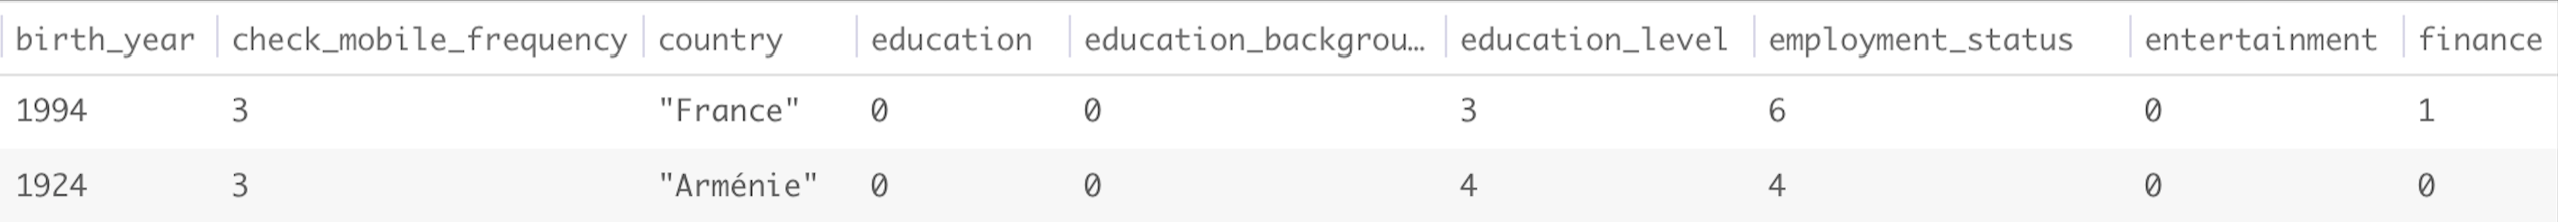
\includegraphics[width=\textwidth,keepaspectratio,height=0.6\textwidth]{./images/collection_ui_1}
\caption{Screenshot of Collection UserInformation Part 1}
\label{fig:col_ui_1}
\end{figure}

\begin{figure}[ht!]
\centering
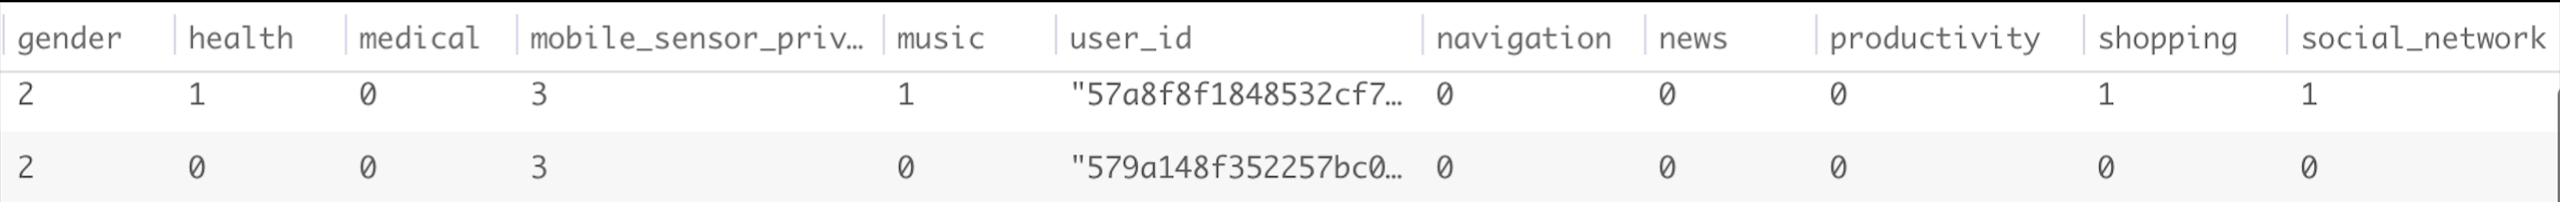
\includegraphics[width=\textwidth,keepaspectratio,height=0.6\textwidth]{./images/collection_ui_2}
\caption{Screenshot of Collection UserInformation Part 2}
\label{fig:col_ui_2}
\end{figure}

\begin{figure}[ht!]
\centering
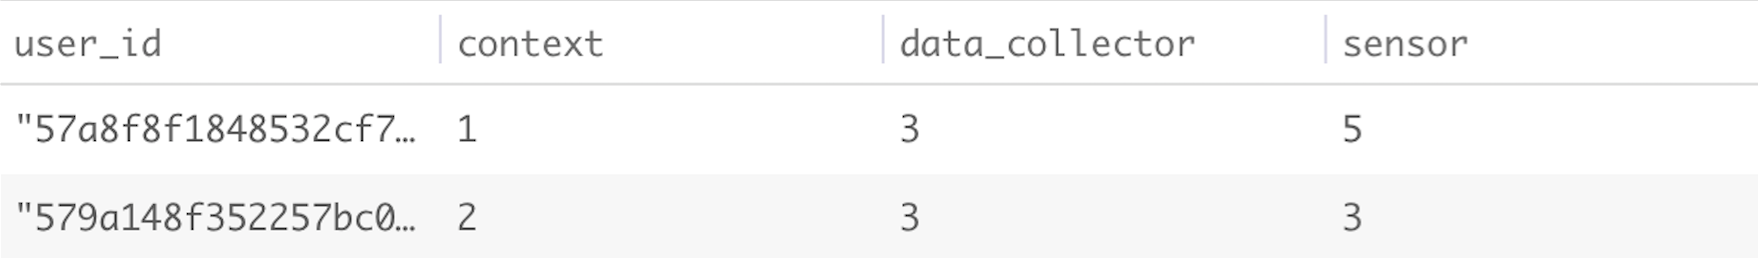
\includegraphics[width=\textwidth,keepaspectratio,height=0.6\textwidth]{./images/collection_feature_cat}
\caption{Screenshot of Collection Features}
\label{fig:col_f}
\end{figure}

\begin{figure}[ht!]
\centering
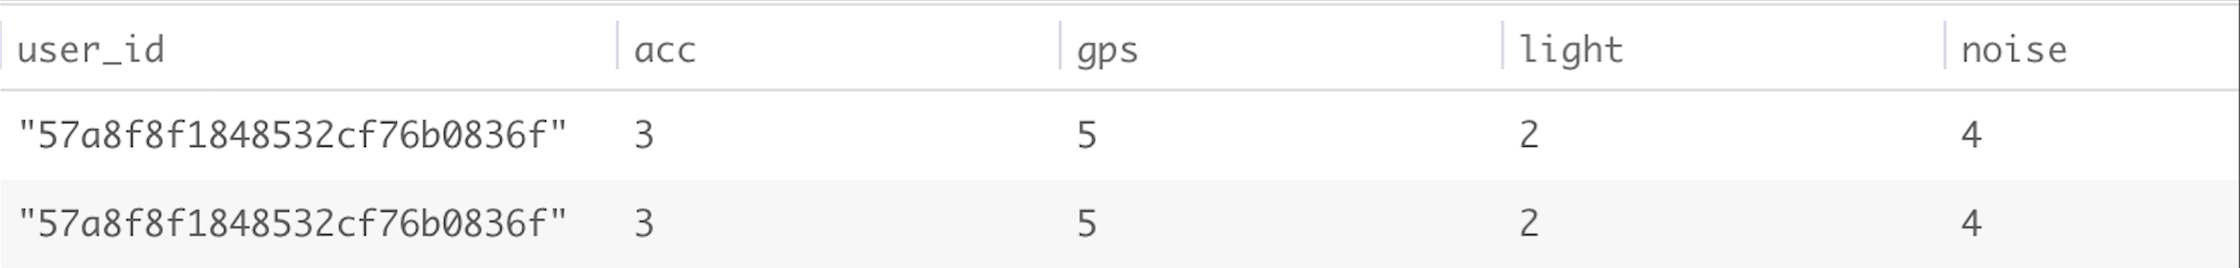
\includegraphics[width=\textwidth,keepaspectratio,height=0.6\textwidth]{./images/collection_sensors_cat}
\caption{Screenshot of Collection Sensors}
\label{fig:col_s}
\end{figure}

\begin{figure}[ht!]
\centering
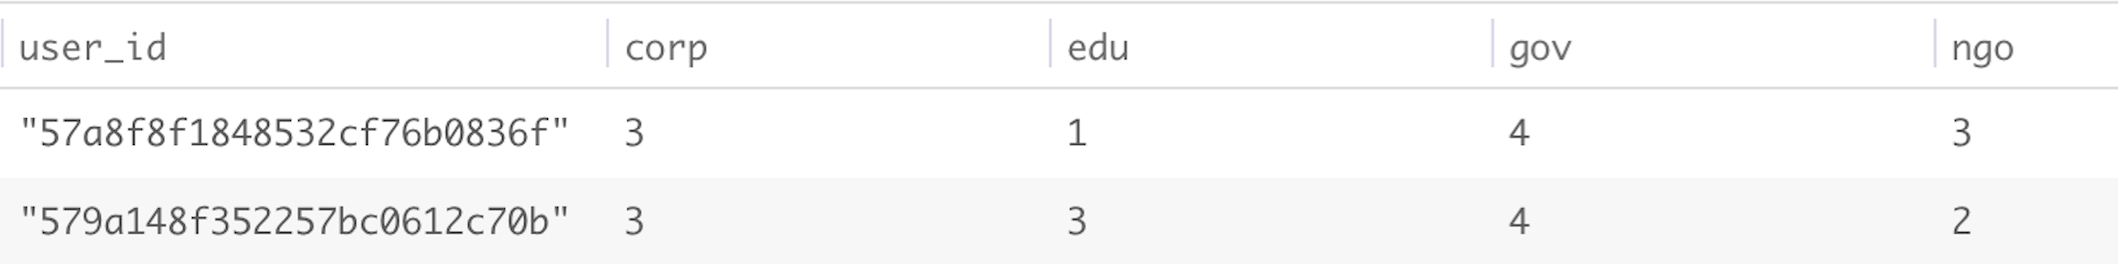
\includegraphics[width=\textwidth,keepaspectratio,height=0.6\textwidth]{./images/collection_dc_cat}
\caption{Screenshot of Collection Stakeholders}
\label{fig:col_ss}
\end{figure}

\begin{figure}[ht!]
\centering
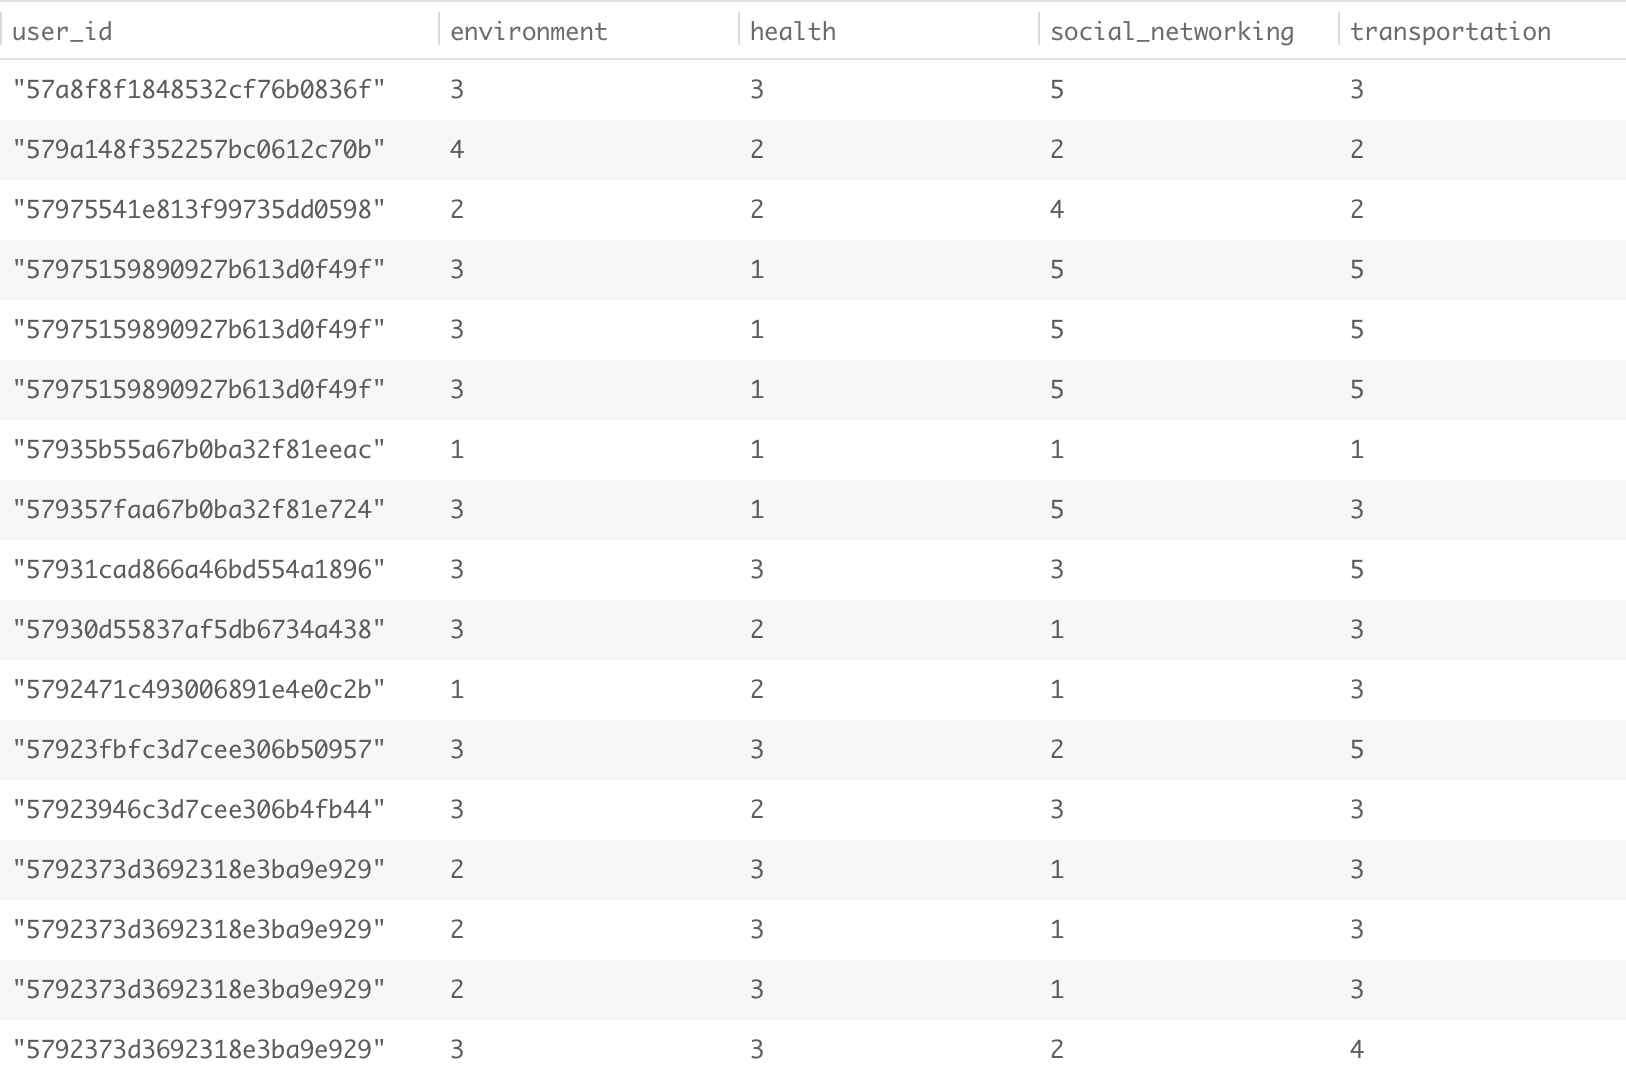
\includegraphics[width=\textwidth,keepaspectratio,height=0.6\textwidth]{./images/collection_context_cat}
\caption{Screenshot of Collection Contexts}
\label{fig:col_c}
\end{figure}

\begin{figure}[ht!]
\centering
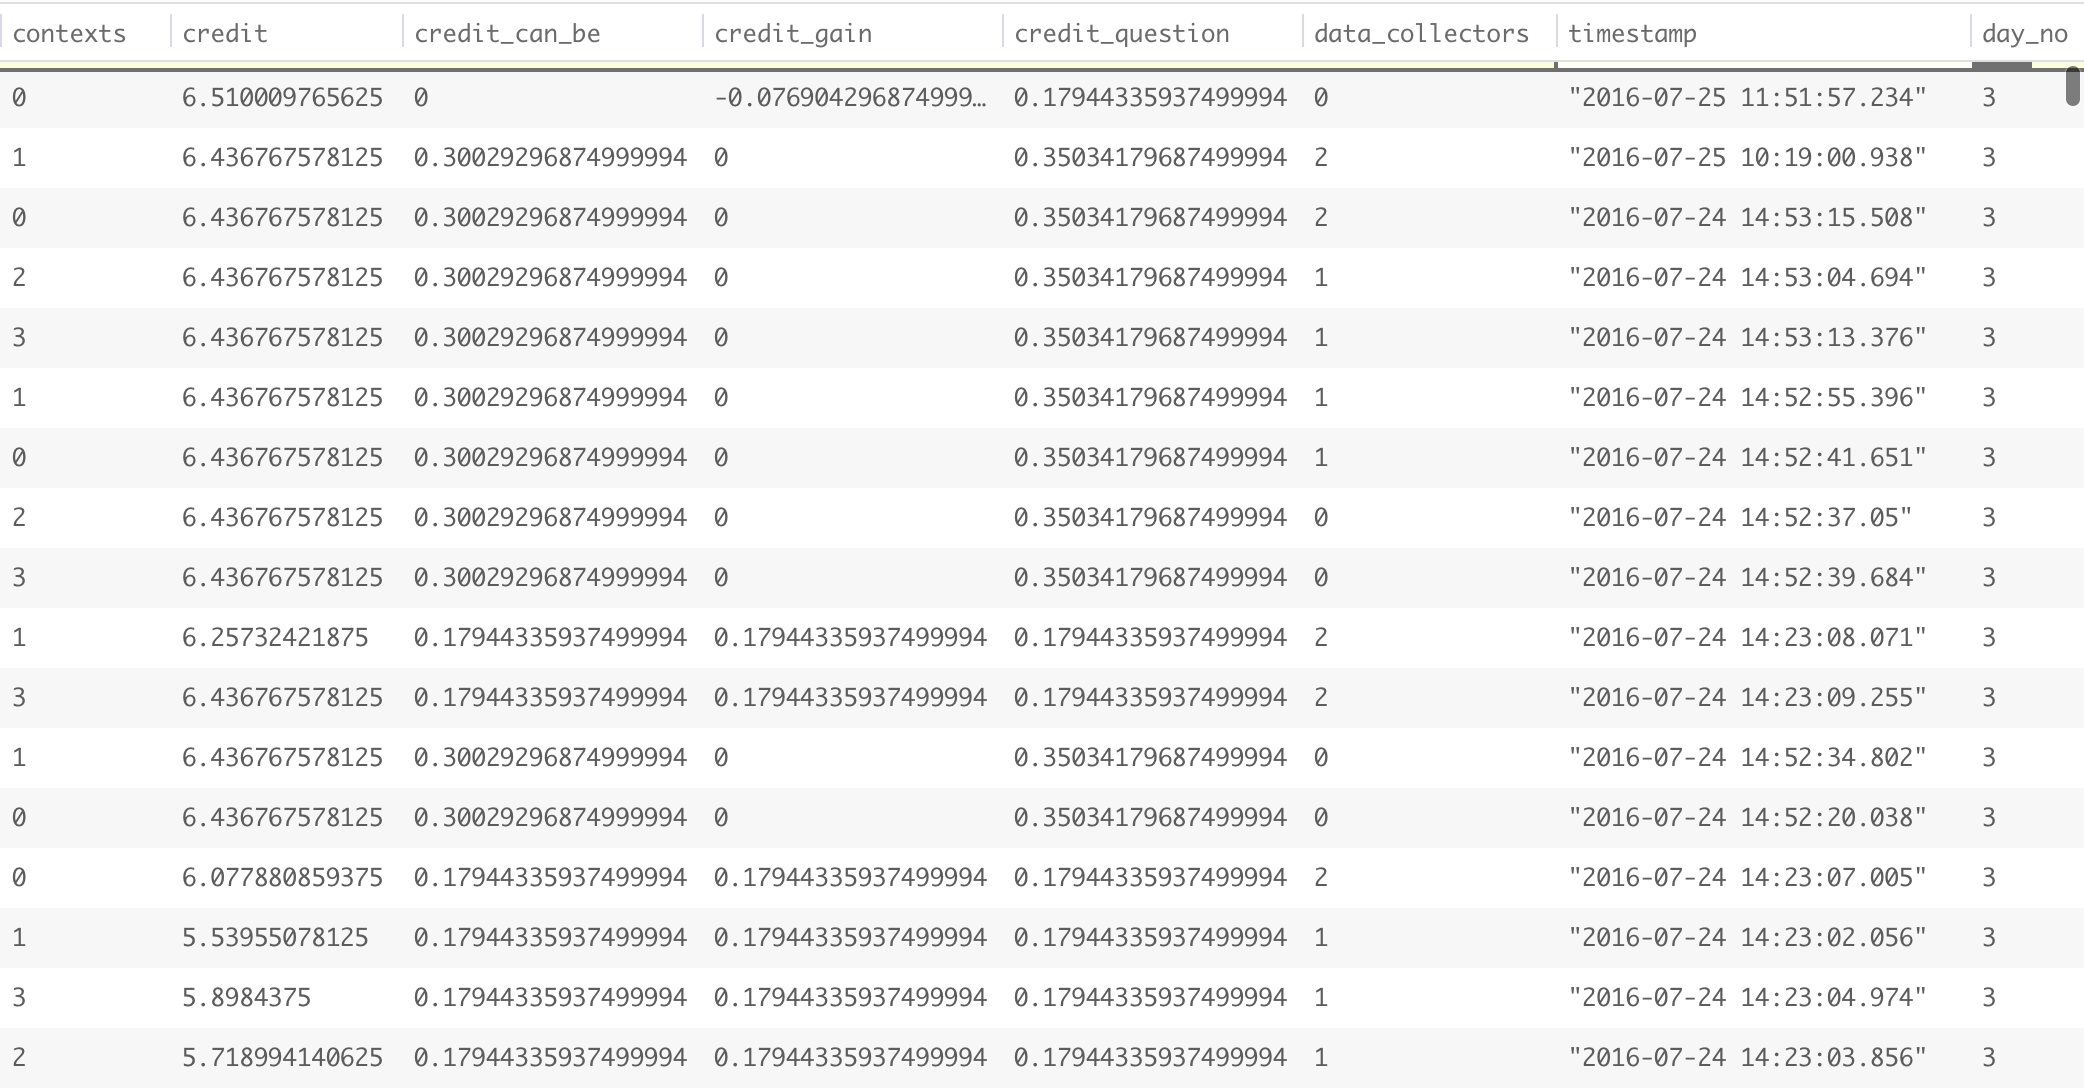
\includegraphics[width=\textwidth,keepaspectratio, height=0.6\textwidth]{./images/collection_ur_1}
\caption{Screenshot of Collection UserResponse Part 1}
\label{fig:col_ur_1}
\end{figure}

\begin{figure}[ht!]
\centering
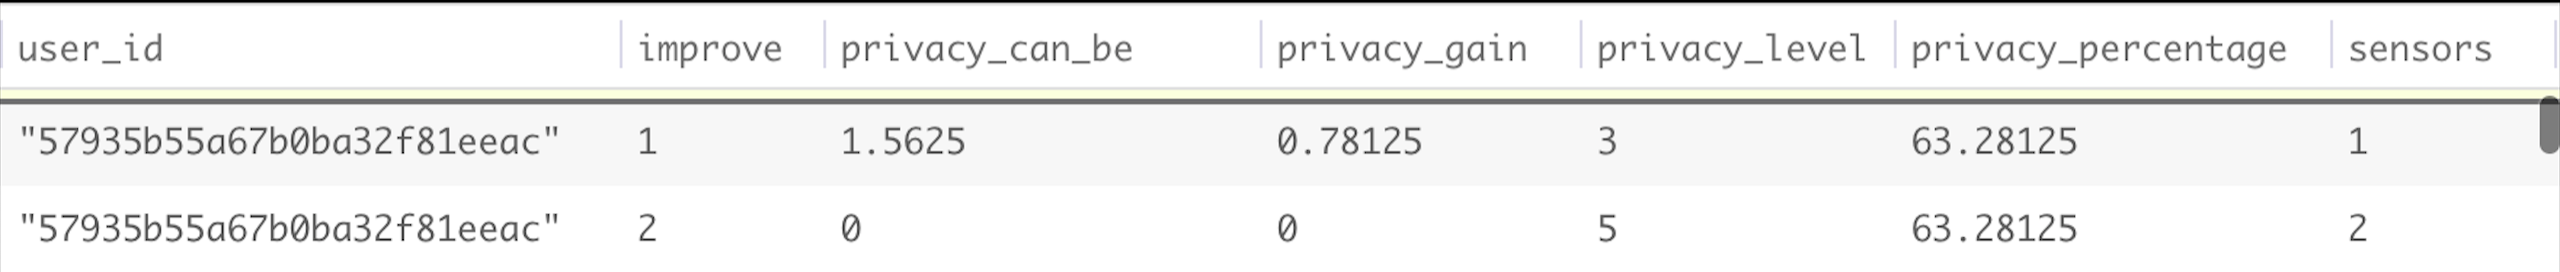
\includegraphics[width=\textwidth,keepaspectratio,height=0.6\textwidth]{./images/collection_ur_2}
\caption{Screenshot of Collection UserResponse Part 2}
\label{fig:col_ur_2}
\end{figure}

\begin{figure}[ht!]
\centering
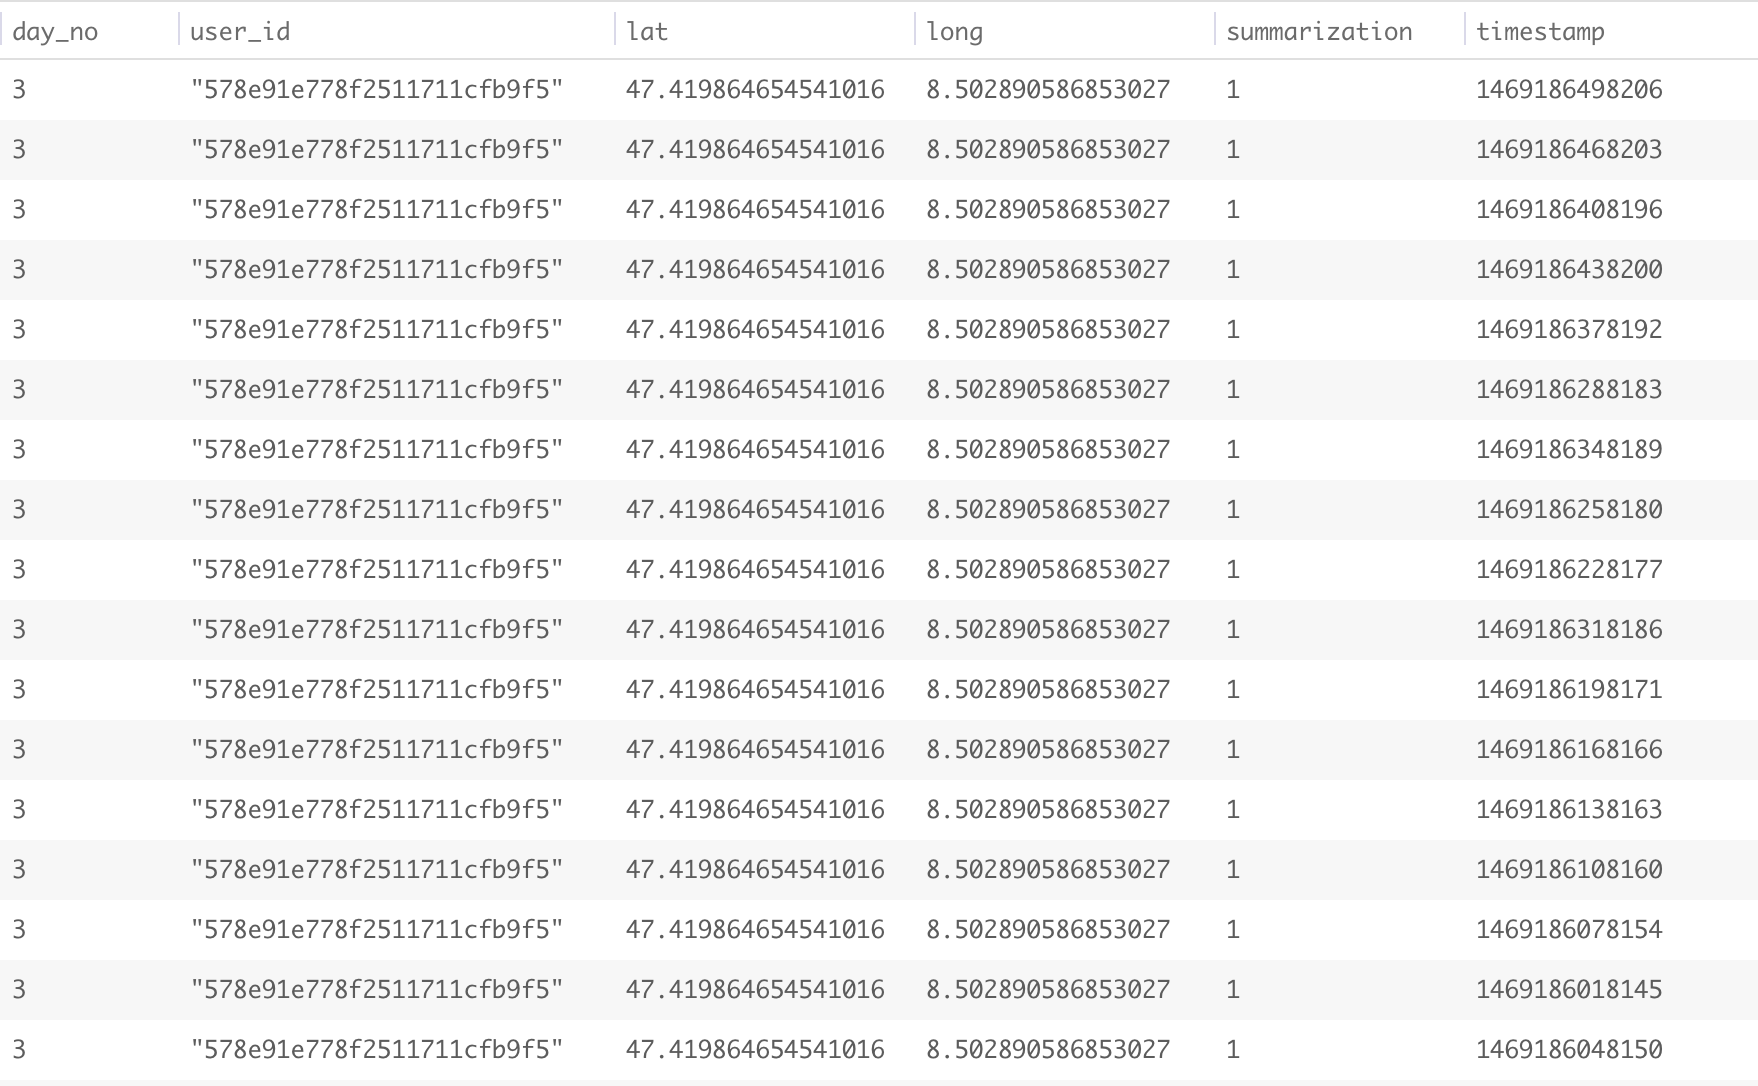
\includegraphics[width=\textwidth,keepaspectratio,height=0.6\textwidth]{./images/collection_loc}
\caption{Screenshot of Collection Location}
\label{fig:col_loc}
\end{figure}

\begin{figure}[ht!]
\centering
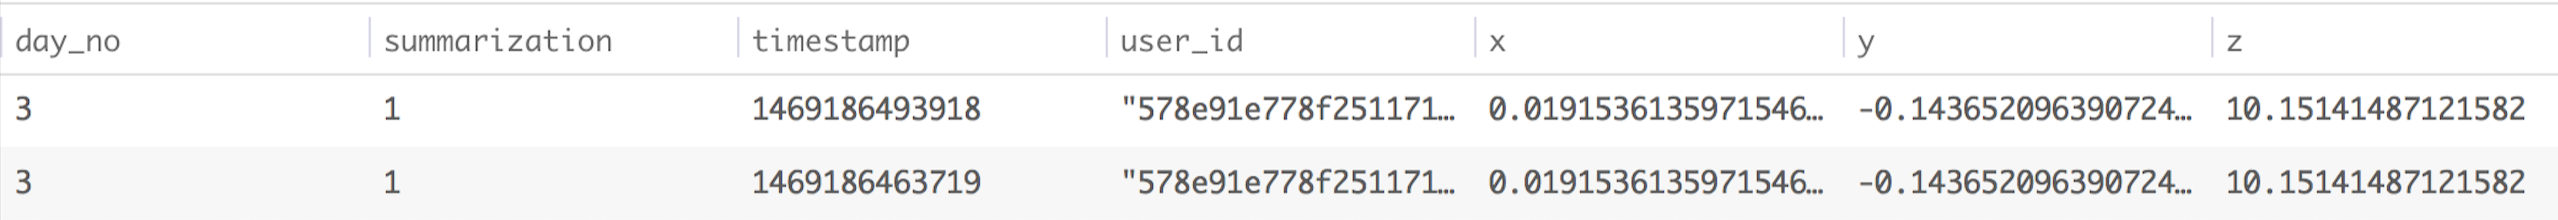
\includegraphics[width=\textwidth,keepaspectratio,height=0.6\textwidth]{./images/collection_acc}
\caption{Screenshot of Collection Accelerometer}
\label{fig:col_acc}
\end{figure}

\begin{figure}[ht!]
\centering
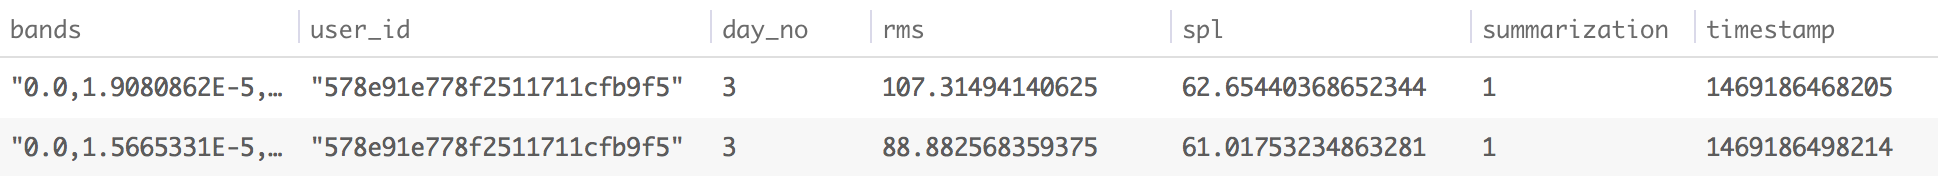
\includegraphics[width=\textwidth,keepaspectratio,height=0.6\textwidth]{./images/collection_noise}
\caption{Screenshot of Collection Noise}
\label{fig:col_noise}
\end{figure}

\begin{figure}[ht!]
\centering
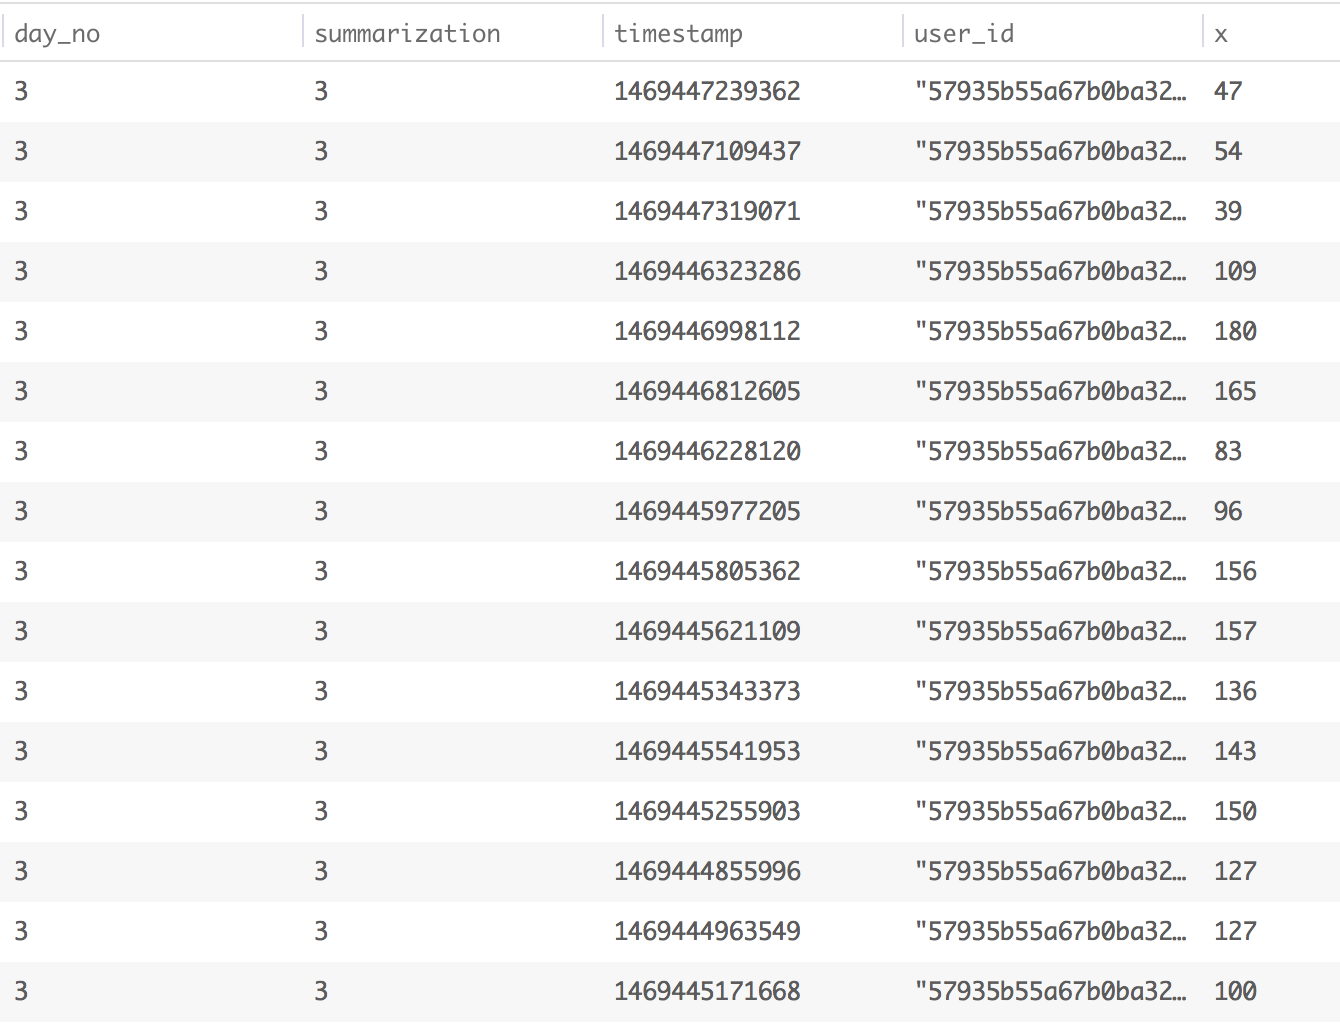
\includegraphics[width=\textwidth,keepaspectratio,height=0.6\textwidth]{./images/collection_light}
\caption{Screenshot of Collection Light}
\label{fig:col_light}
\end{figure}

\begin{figure}[ht!]
\centering
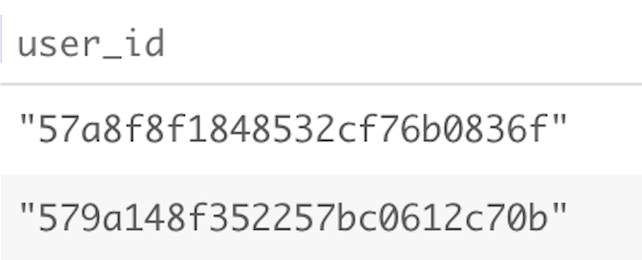
\includegraphics[width=\textwidth,keepaspectratio,height=0.6\textwidth]{./images/collection_users}
\caption{Screenshot of Collection Users}
\label{fig:col_users}
\end{figure}

\begin{figure}[ht!]
\centering
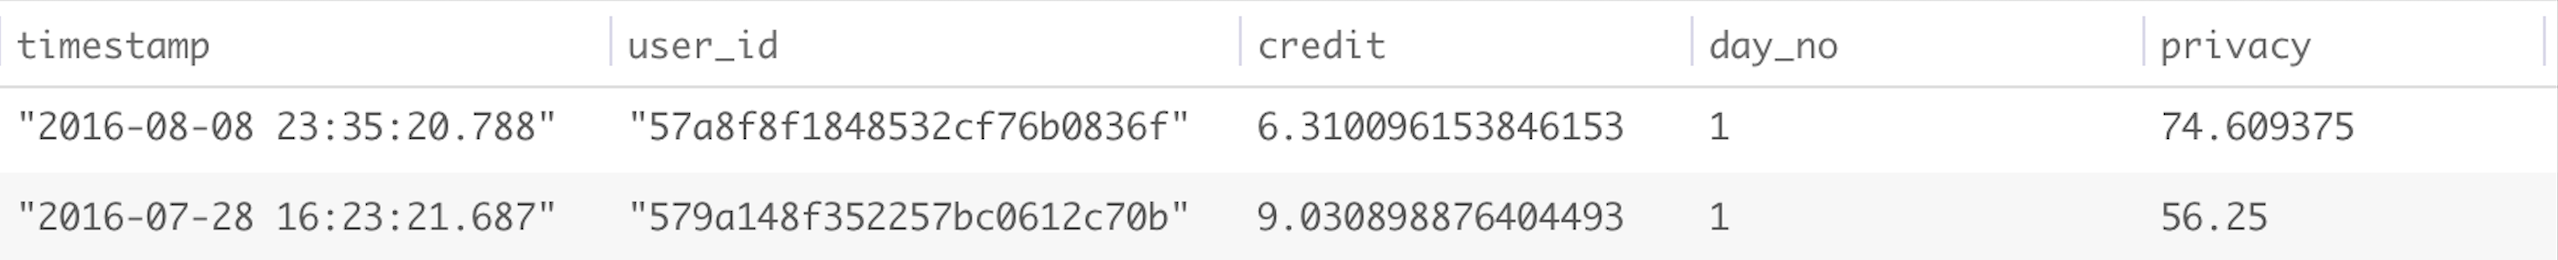
\includegraphics[width=\textwidth,keepaspectratio,height=0.6\textwidth]{./images/collection_score}
\caption{Screenshot of Collection Score}
\label{fig:col_score}
\end{figure}

\chapter{Appendix B}

\begin{table}[h!]
  \centering
  \caption{Demographics of Population in the Survey}
  \label{tab:demo}
  \begin{tabular}{cc}
    \toprule
     Country&Percentage\\
    \midrule
United States of America&1.01\%\\
United Arab Emirates&0.51\%\\
The former Yugoslav Republic of Macedonia&0.51\%\\
Syrian Arab Republic	&0.51\%\\
Switzerland&20.71\%\\
Spain	&1.01\%\\
Slovakia	&0.51\%\\
Serbia&	5.05\%\\
Russian Federation&	0.51\%\\
Netherlands	&1.52\%\\
Italy	&2.02\%\\
Iran&1.01\%\\
India	&14.65\%\\
Hungary	&0.51\%\\
Greece	&29.29\%\\
Germany	&10.61\%\\
France	&1.52\%\\
Czech Republic	&1.01\%\\
Costa Rica	&0.51\%\\
China	&0.51\%\\
Columbia	&0.51\%\\
Canada	&0.51\%\\
Bolivia	&0.51\%\\
Brazil	&1.52\%\\
Bahrain	&0.51\%\\
Argentina	&0.51\%\\
Austria & 2.02\%\\
    \bottomrule
  \end{tabular}
\end{table}

%\begin{table}[h!]
%  \centering
%  \caption{Employment Classification of Groups For Sensors}
%  \label{tab:emp_sensors}
%  \begin{tabular}{cccccc}
%    \toprule
%     Occupation&1&2&3&4&5\\
%    \midrule
%Employed full time&4.90\%&6.86\%&26.47\%&38.24\%&23.53\%\\
%Employed part time&8.33\%&16.67\%&33.33\%&16.67\%&25.00\%\\
%Unemployed and looking for work&8.33\%&16.67\%&16.67\%&25.00\%&33.33\%\\
%Unemployed and not looking for work&0.00\%&0.00\%&0.00\%&66.67\%&33.33\%\\
%Retired&0.00\%&0.00\%&100.00\%&0.00\%&0.00\%\\
%Student&7.23\%&4.82\%&26.51\%&39.76\%&21.69\%\\
%Disabled&0.00\%&0.00\%&0.00\%&0.00\%&0.00\%\\
%    \bottomrule
%  \end{tabular}
%\end{table}
%
%
%
%\begin{table}[h!]
%  \centering
%  \caption{Gender Classification of Groups For Sensors}
%  \label{tab:gender_sensors}
%  \begin{tabular}{cccccc}
%    \toprule
%     Gender&1&2&3&4&5 \\
%    \midrule
%Female&5.56\%&4.17\%&33.33\%&30.56\%&26.39\% \\
%Male&7.14\%&9.52\%&22.22\%&39.68\%&21.43\% \\
%    \bottomrule
%  \end{tabular}
%\end{table}
%
%
%
%\begin{table}[h!]
%  \centering
%  \caption{Average Birth Year of Groups For Sensors}
%  \label{tab:year_sensors}
%  \begin{tabular}{ccccc}
%    \toprule
%     1&2&3&4&5\\
%    \midrule
%	1989& 1979& 1986& 1986& 1983\\
%    \bottomrule
%  \end{tabular}
%\end{table}
%
%
%\begin{table}[h!]
%  \centering
%  \caption{Education Classification of Groups For Sensors}
%  \label{tab:edu_sensors}
%  \begin{tabular}{cccccc}
%    \toprule
%     Education&1&2&3&4&5\\
%    \midrule
%    
%Less than high school&20.00\%&20.00\%&20.00\%&40.00\%&0.00\%\\
%High school&10.53\%&0.00\%&52.63\%&31.58\%&5.26\%\\
%Some college&10.00\%&20.00\%&30.00\%&20.00\%&20.00\%\\
%Bachelors degree&7.02\%&10.53\%&24.56\%&42.11\%&15.79\%\\
%Masters degree&3.80\%&5.06\%&24.05\%&35.44\%&31.65\%\\
%PhD degree&7.14\%&7.14\%&17.86\%&35.71\%&32.14\%\\
%    \bottomrule
%  \end{tabular}
%\end{table} 
%
%
%
%
%
%
%
%
%
%
%\begin{table}[h!]
%  \centering
%  \caption{Employment Classification of Groups For Stakeholders}
%  \label{tab:emp_stak}
%  \begin{tabular}{cccccc}
%    \toprule
%     Occupation&1&2&3&4&5\\
%    \midrule
%Employed full time	&3.92\%	&4.90\%	&16.67\%	&33.33\%	&41.18\%\\
%Employed part time	&16.67\%	&16.67\%	&8.33\%	&50.00\%	&8.33\%\\
%Unemployed, looking for work	&8.33\%	&8.33\%	&16.67\%	&16.67\%	&50.00\%\\
%Unemployed, not looking for work	&0.00\%	&0.00\%	&0.00\%	&33.33\%	&66.67\%\\
%Retired	&0.00\%	&0.00\%	&0.00\%	&100.00\%&	0.00\%\\
%Student	&4.82\%	&7.23\%	&15.66\%	&37.35\%	&34.94\%\\
%Disabled	&0.00\%	&0.00\%	&0.00\%	&0.00\%	&0.00\%\\
%    \bottomrule
%  \end{tabular}
%\end{table}
%
%
%
%\begin{table}[h!]
%  \centering
%  \caption{Gender Classification of Groups For Stakeholders}
%  \label{tab:gender_stak}
%  \begin{tabular}{cccccc}
%    \toprule
%     Gender&1&2&3&4&5 \\
%     \midrule
%Female&5.56\%&6.94\%&23.61\%&36.11\%&27.78\% \\
%Male&3.97\%&6.35\%&11.90\%&35.71\%&42.06\%\\
%    \bottomrule
%  \end{tabular}
%\end{table}
%
%
%
%\begin{table}[h!]
%  \centering
%  \caption{Average Birth Year of Groups For Stakeholders}
%  \label{tab:year_stak}
%  \begin{tabular}{ccccc}
%    \toprule
%     1&2&3&4&5\\
%    \midrule
%	1986& 1989& 1984& 1985& 1984\\
%    \bottomrule
%  \end{tabular}
%\end{table}
%
%
%\begin{table}[h!]
%  \centering
%  \caption{Education Classification of Groups For Stakeholders}
%  \label{tab:edu_stak}
%  \begin{tabular}{cccccc}
%    \toprule
%     Education&1&2&3&4&5\\
%    \midrule
%    
%Less than high school	&20.00\%	&20.00\%	&0.00\%	&60.00\%	&0.00\%\\
%High school	& 15.79\%&	5.26\%	&21.05\%	&31.58\%	&26.32\%\\
%Some college	 & 0.00\%&	10.00\%	&20.00\%	&40.00\%&	30.00\%\\
%Bachelors degree 	&1.75\%	&12.28\%&	15.79\%	&35.09\%	&35.09\%\\
%Masters degree	&5.06\%	&1.27\%	&13.92\%	&37.97\%	&41.77\%\\
%PhD degree	&0.00\%	&7.14\%	&21.43\%	&28.57\%	&42.86\%\\
%    \bottomrule
%  \end{tabular}
%\end{table}
%
%
%
%
%
%
%
%
%\begin{table}[h!]
%  \centering
%  \caption{Employment Classification of Groups For Contexts}
%  \label{tab:emp_c}
%  \begin{tabular}{cccccc}
%    \toprule
%     Occupation&1&2&3&4&5\\
%    \midrule
%Employed full time	&4.90\%	&3.92\%	&23.53\%	&36.27\%	&31.37\%\\
%Employed part time	&16.67\%	&8.33\%	&25.00\%	&25.00\%	&25.00\%\\
%Unemployed, looking for work	&8.33\%	&16.67\%	&25.00\%	&25.00\%	&25.00\%\\
%Unemployed, not looking for work	&0.00\%	&0.00\%	&0.00\%	&66.67\%	&33.33\%\\
%Retired	&0.00\%	&0.00\%	&0.00\%	&100.00\% &	0.00\%\\
%Student	&7.23\%	&6.02\%	&20.48\%	&44.58\%	&21.69\%\\
%Disabled	&0.00\%	&0.00\%	&0.00\%	&0.00\%	&0.00\%\\
%    \bottomrule
%  \end{tabular}
%\end{table}
%
%
%
%\begin{table}[h!]
%  \centering
%  \caption{Gender Classification of Groups For Contexts}
%  \label{tab:gender_c}
%  \begin{tabular}{cccccc}
%    \toprule
%     Gender&1&2&3&4&5 \\
%    \midrule
%Male&	7.14\%	&6.35\%	&23.02\%	&38.10\%	&25.40\% \\
%Female	&5.56\%	&5.56\%	&19.44\%	&38.89\%	&30.56\% \\
%    \bottomrule
%  \end{tabular}
%\end{table}
%
%
%
%\begin{table}[h!]
%  \centering
%  \caption{Average Birth Year of Groups For Contexts}
%  \label{tab:year_c}
%  \begin{tabular}{ccccc}
%    \toprule
%     1&2&3&4&5\\
%    \midrule
%	1986& 1986& 1986& 1985& 1983\\
%    \bottomrule
%  \end{tabular}
%\end{table}
%
%
%\begin{table}[h!]
%  \centering
%  \caption{Education Classification of Groups For Contexts}
%  \label{tab:edu_c}
%  \begin{tabular}{cccccc}
%    \toprule
%     Education&1&2&3&4&5\\
%    \midrule
%    
%Less than high school	&20.00\%	&0.00\%	&0.00\%	&80.00\%	&0.00\%\\
%High school	&10.53\%	&10.53\%	&31.58\%	&36.84\%	&10.53\%\\
%Some college	1&0.00\%	&0.00\%	&40.00\%	&30.00\%	&20.00\%\\
%Bachelors degree	&7.02\%	&8.77\%	&24.56\%	&35.09\%	&24.56\%\\
%Masters degree	&6.33\%	&3.80\%	&17.72\%	&40.51\%	&31.65\%\\
%PhD degree	&0.00\%	&7.14\%	&17.86\%	&35.71\%	3&9.29\%\\
%    \bottomrule
%  \end{tabular}
%\end{table} 

\chapter{Appendix C}

%\begin{figure}[ht!]
%\centering
%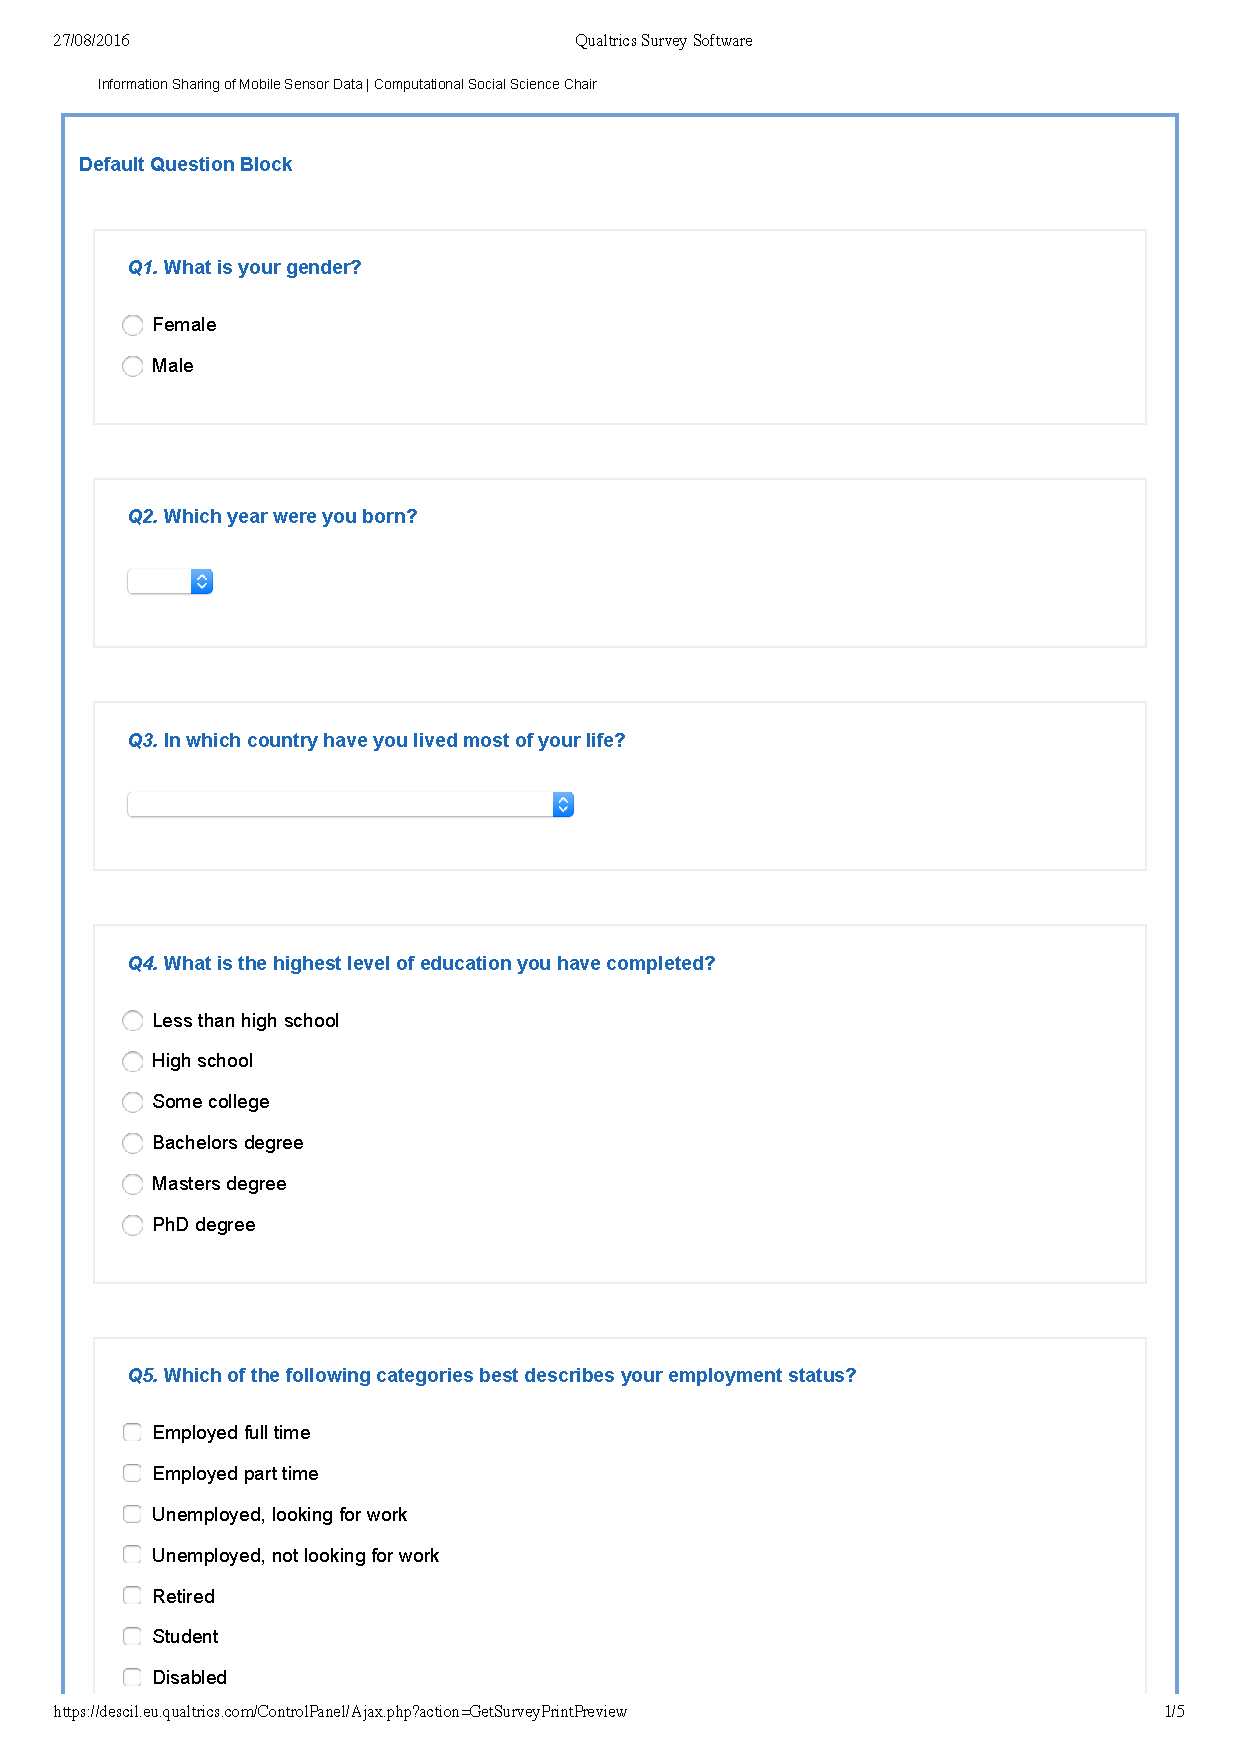
\includegraphics[width=\textwidth,keepaspectratio,height=0.6\textwidth]{pre-survey-pdf}
%\caption{Screenshot of Collection UserInformation Part 2}
%\label{fig:col_ui_2}
%\end{figure}
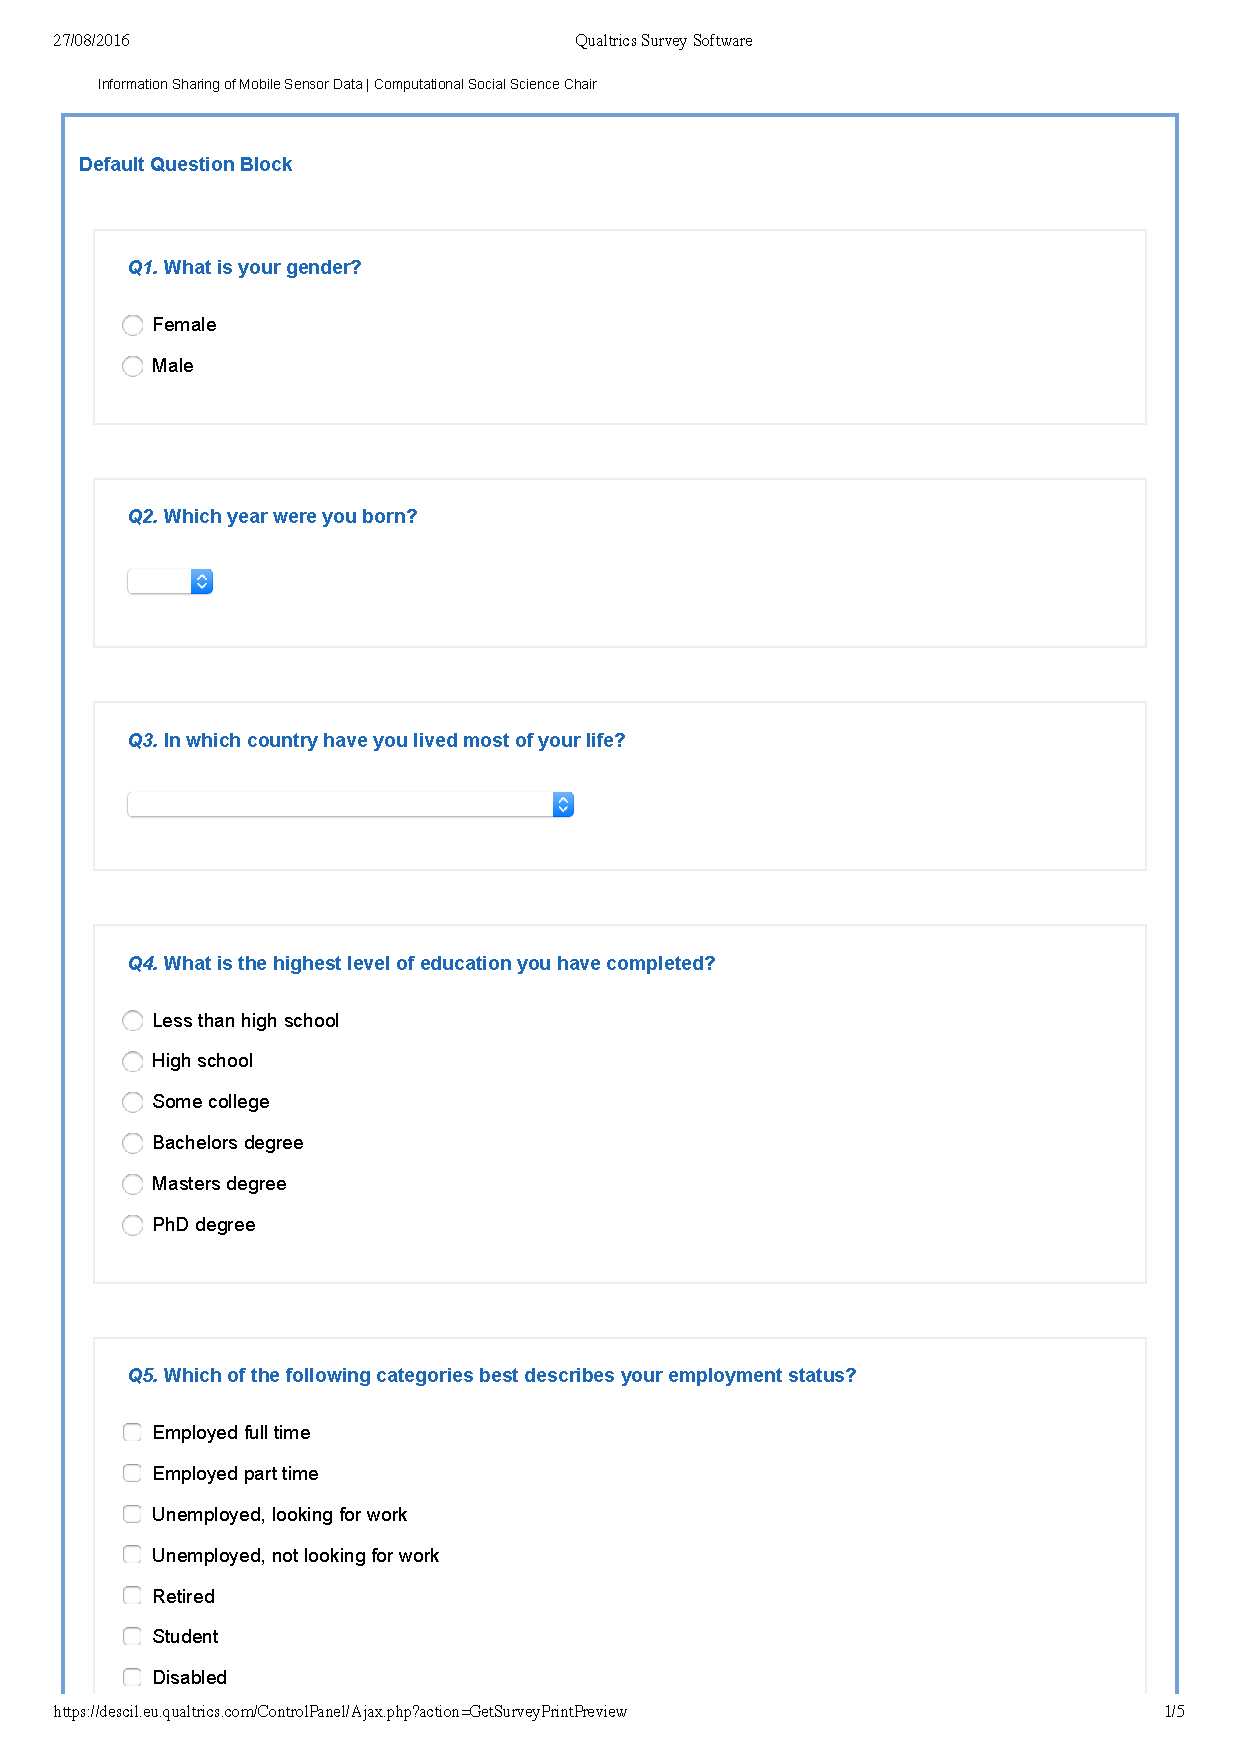
\includepdf[scale=0.6,pages={1},pagecommand=\section*{Pre-Survey \label{app:pre_survey}}]{pre-survey-pdf}
\includepdf[scale=0.6,pages={2-}]{pre-survey-pdf}
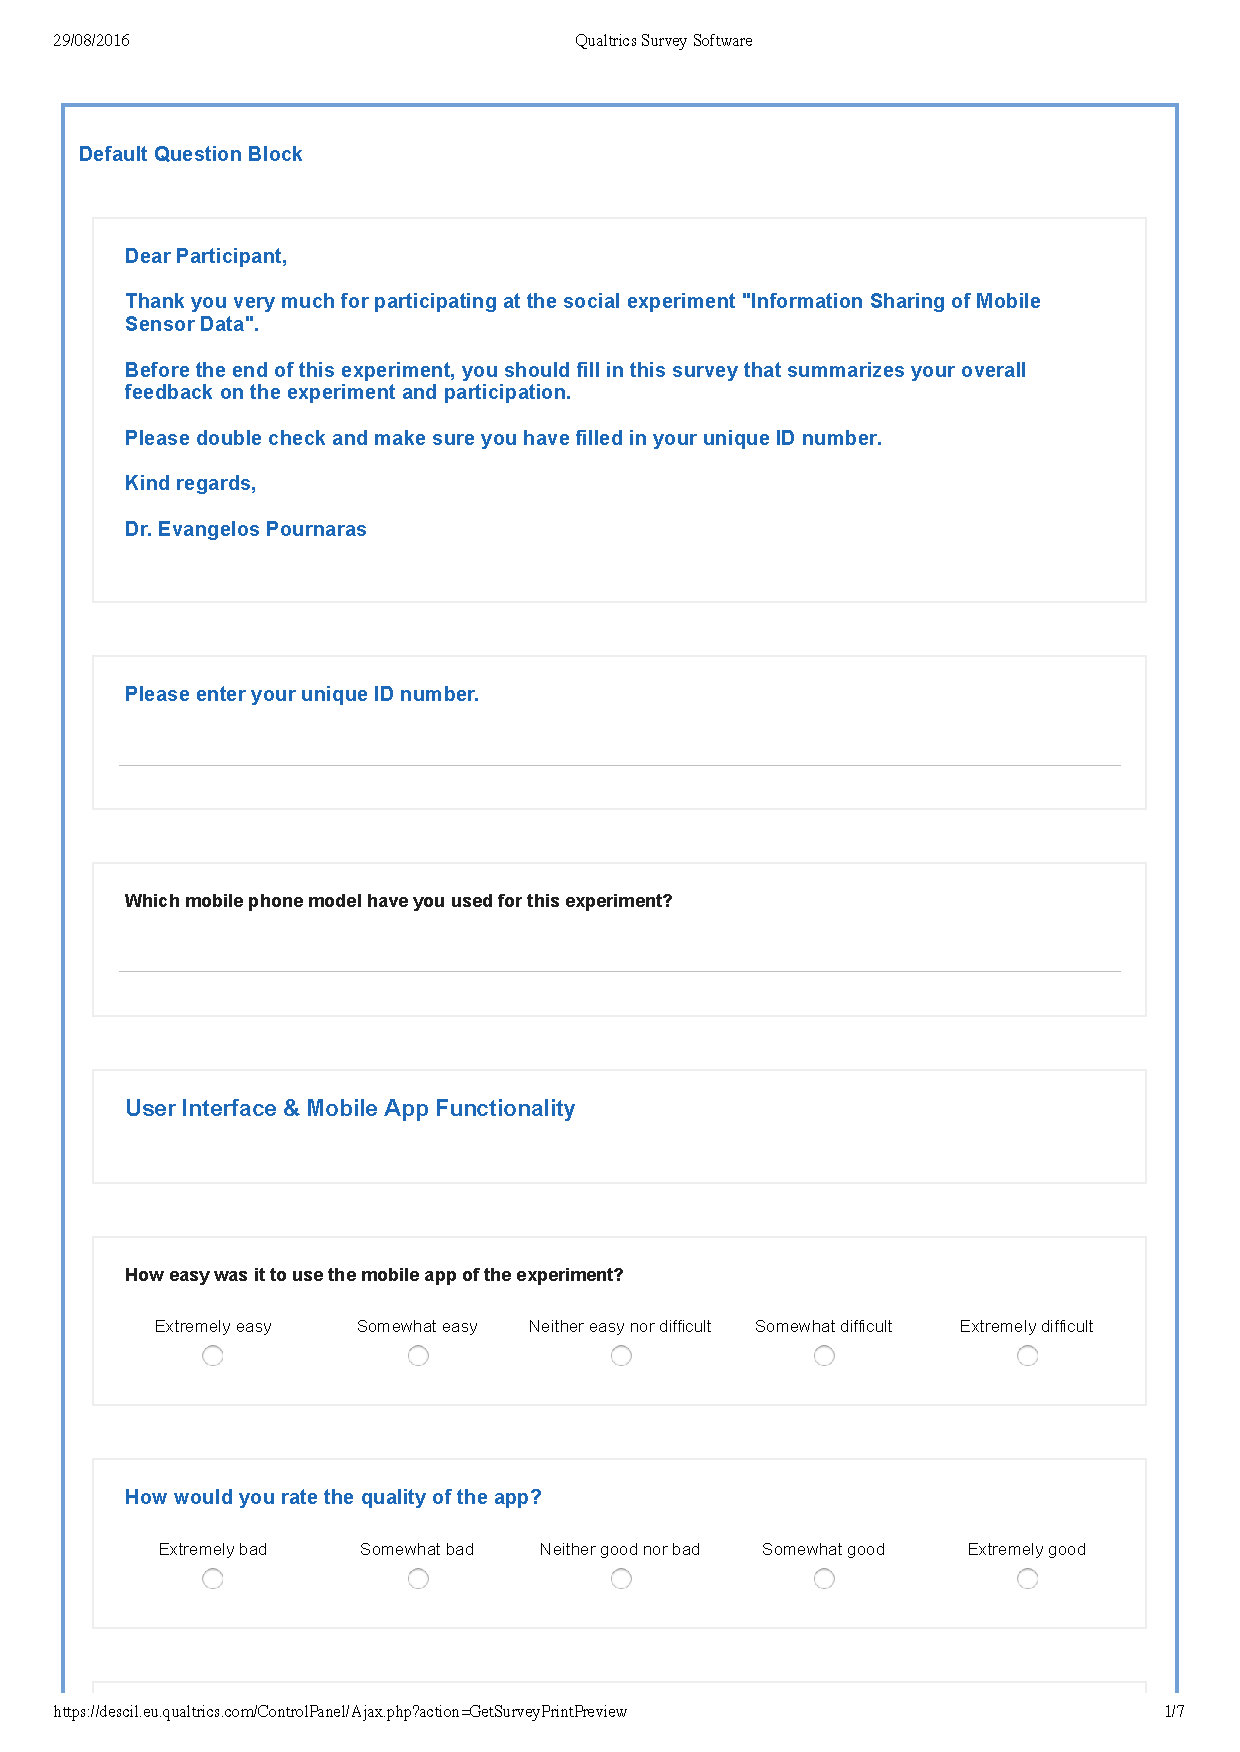
\includepdf[scale=0.6,pages={1},pagecommand=\section*{Exit-Survey \label{app:exit_survey}}]{exit-survey}
\includepdf[scale=0.6,pages={2-}]{exit-survey}
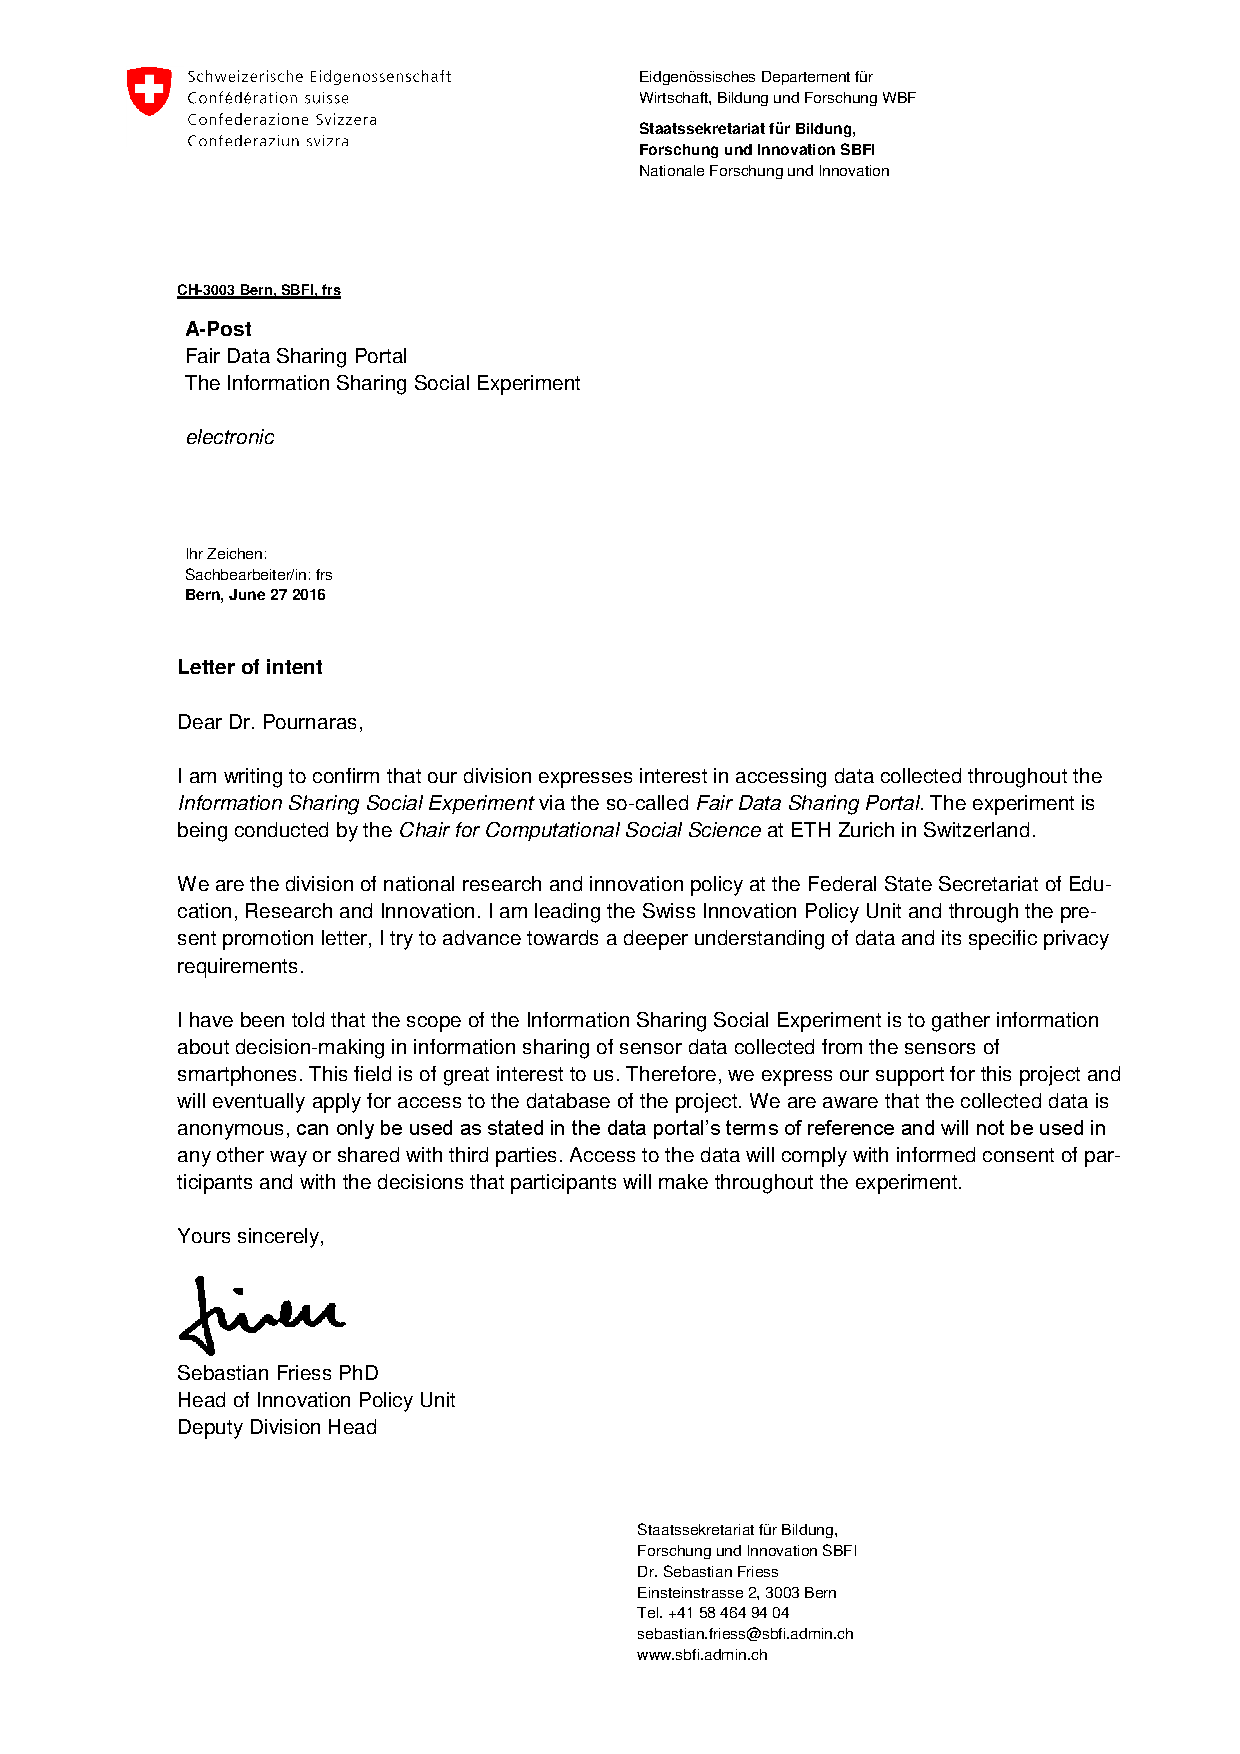
\includepdf[scale=0.6,pages={-},pagecommand=\section*{Support Letters \label{app:supp}}]{co-1}

\includepdf[scale=0.6,pages={-}]{co-2}
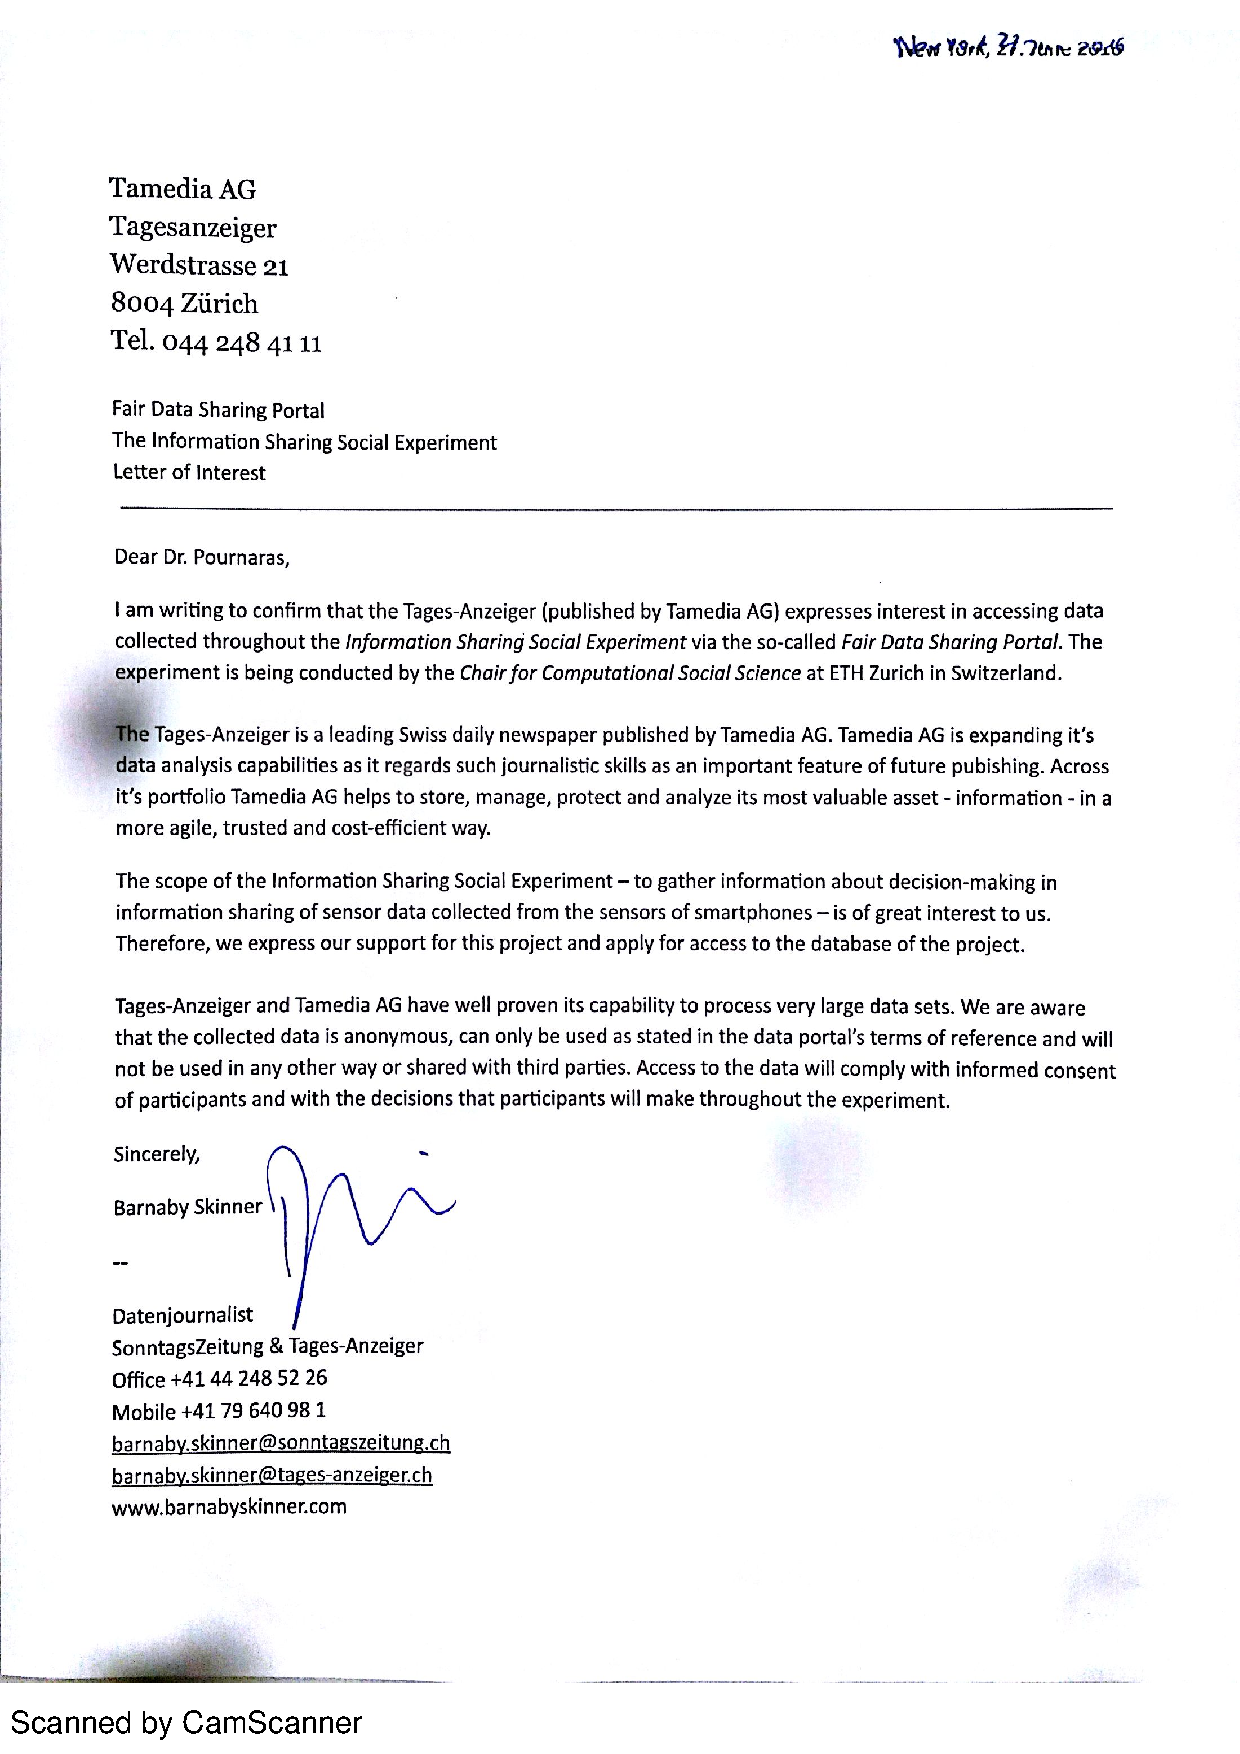
\includepdf[scale=0.6,pages={-}]{co-3}
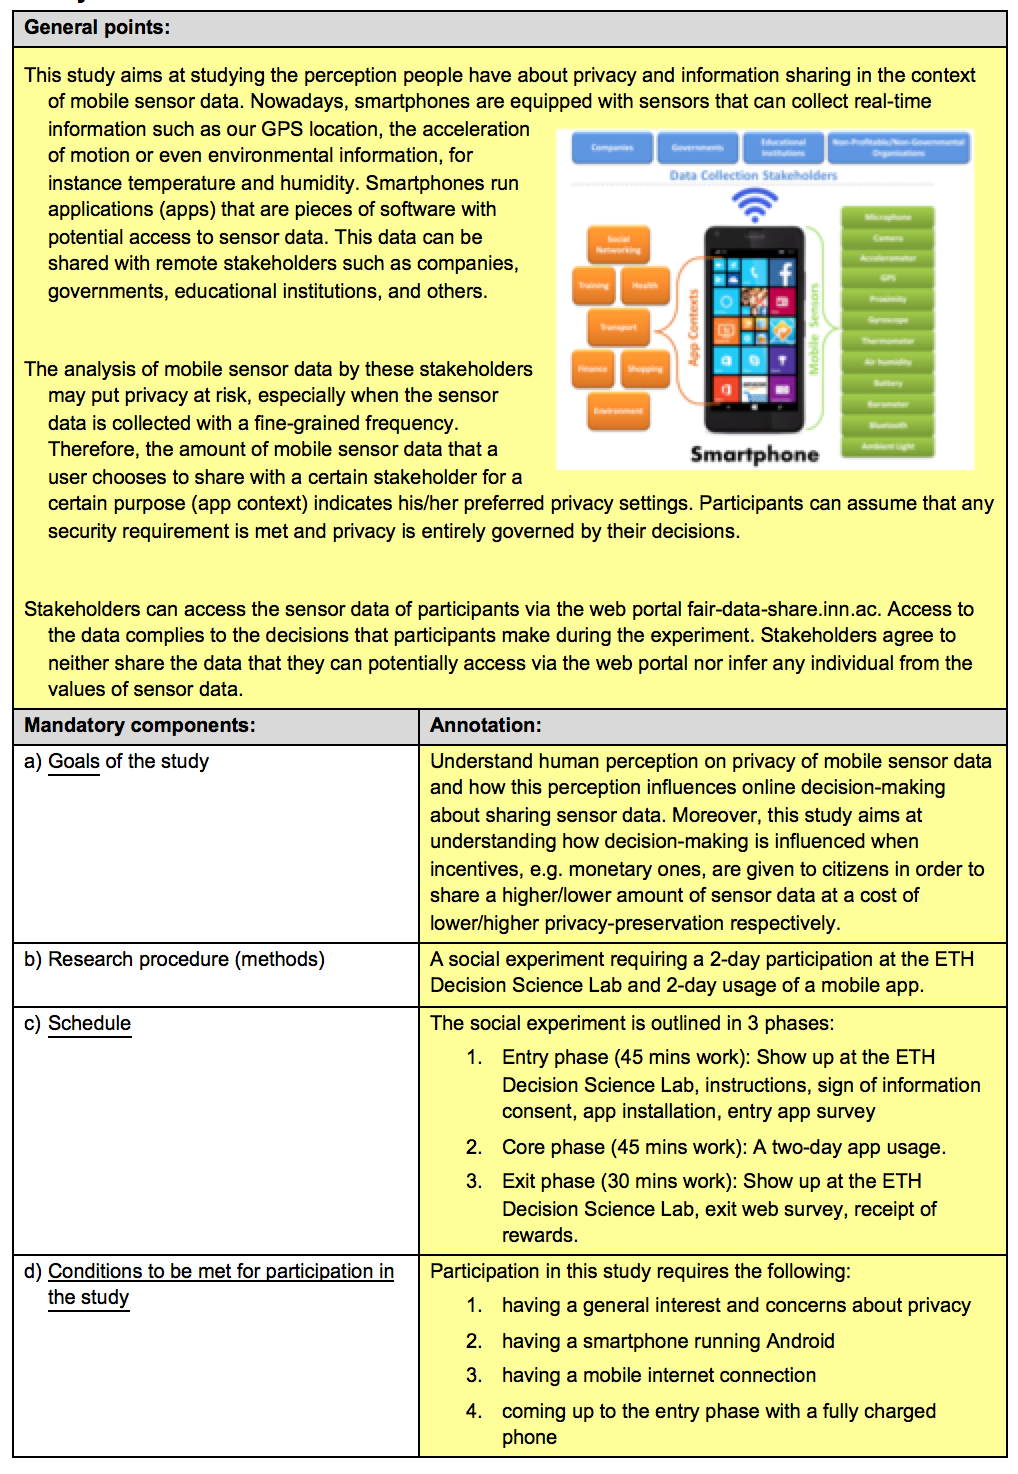
\includepdf[scale=0.6,pages={-},pagecommand=\section*{Information Sheet\label{app:inf}}]{inf-1}
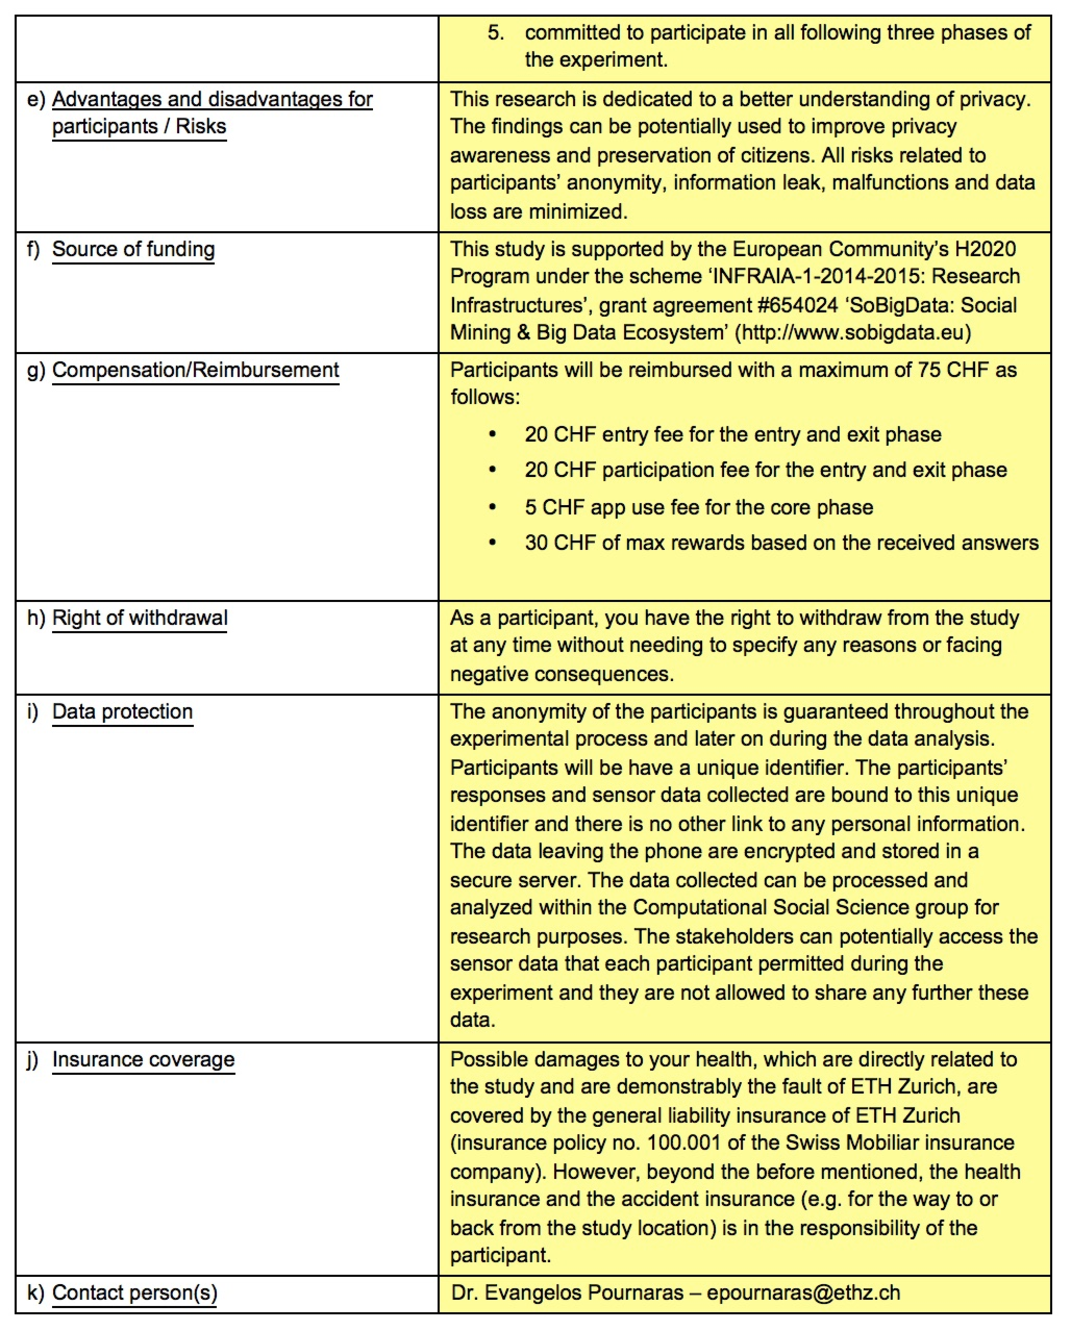
\includepdf[scale=0.6,pages={-}]{inf-2}
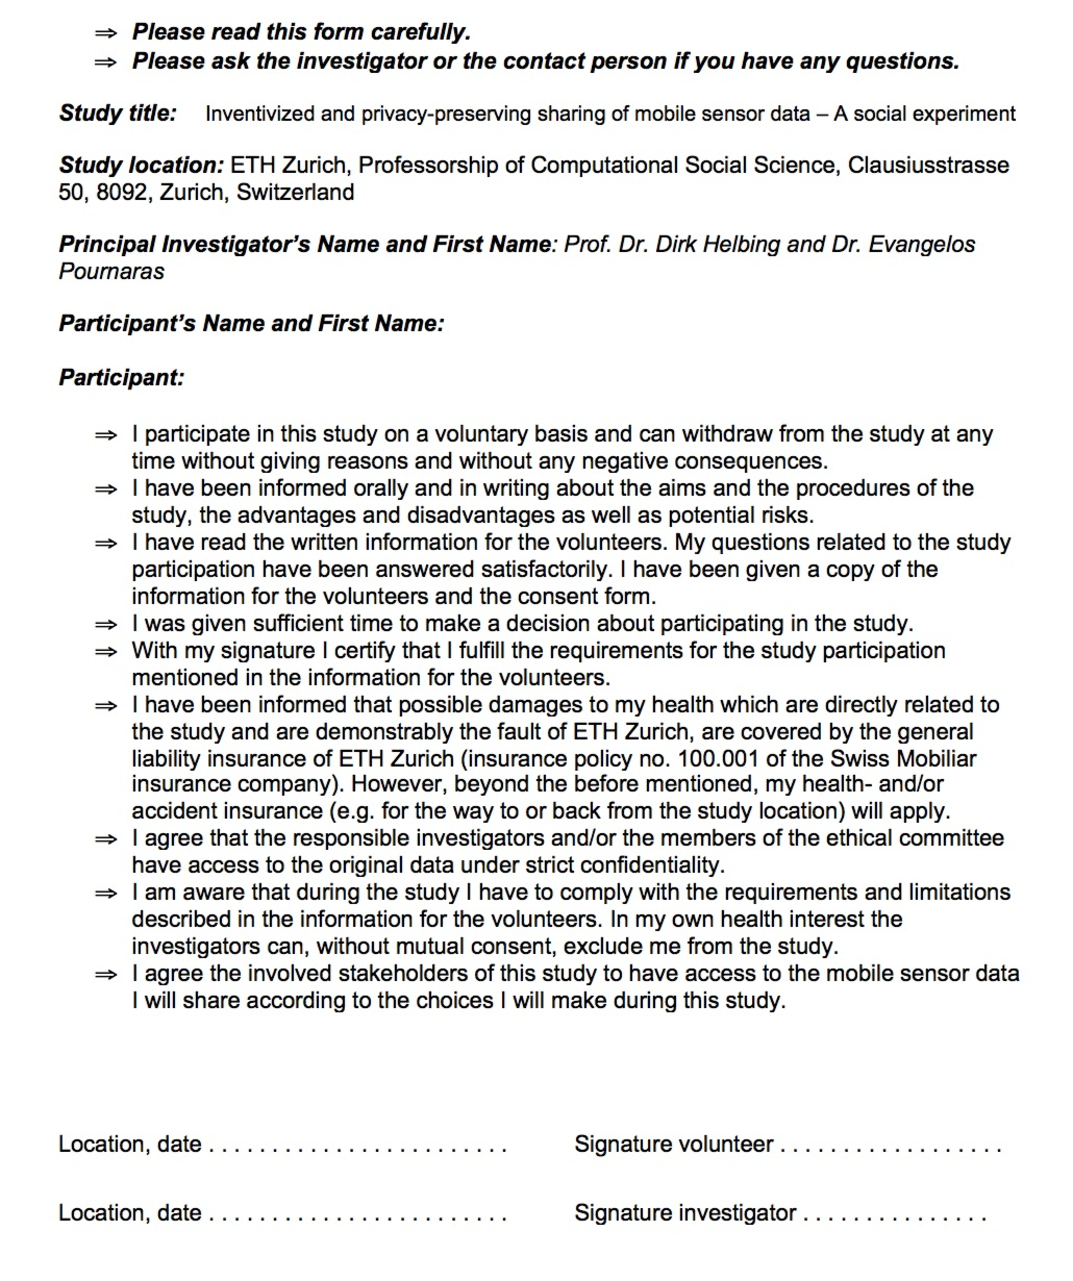
\includepdf[scale=0.6,pages={-},pagecommand=\section*{Consent Form\label{app:consent}}]{consent}